\section{Contention aware Connected Dominating Set (CACDS) Construction Algorithm}
A brief description of the proposed algorithms is stated in this section. The first algorithm is a centralized one because it needs the global topology information of a network for constructing CDS and the second one is the distributed algorithm where each node knows only its two hop neighborhood information.   

\begin{figure*}[h]
\begin{minipage}{.25\textwidth}
\centering
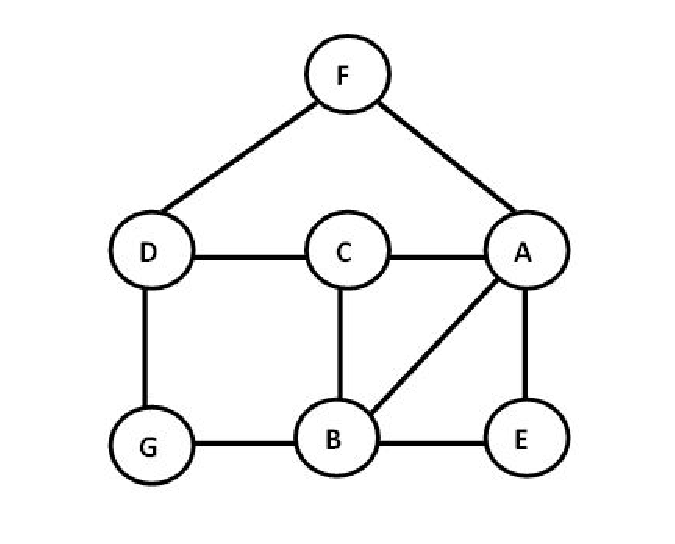
\includegraphics[width=0.9\linewidth,height=.8\linewidth]{Figures/cacds1.eps}
\\(a): All nodes are colored WHITE
\end{minipage}%
\begin{minipage}{.25\textwidth}
\centering
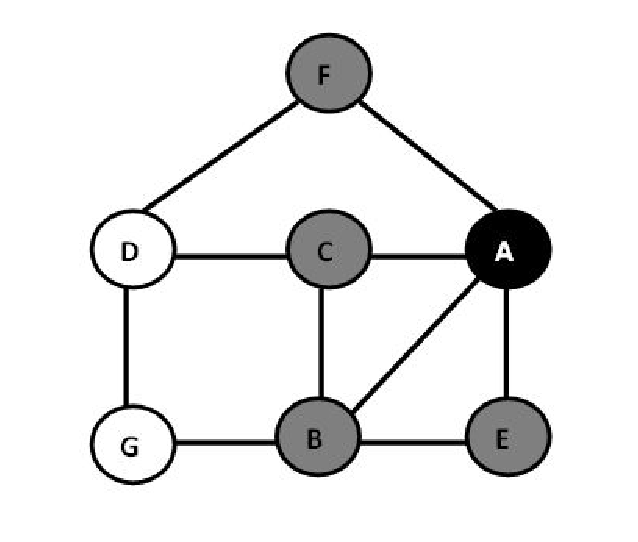
\includegraphics[width=0.9\linewidth,height=.8\linewidth]{Figures/cacds2.eps}
\\(b): Node A is selected and colored BLACK
\end{minipage}%
\begin{minipage}{.25\textwidth}
\centering
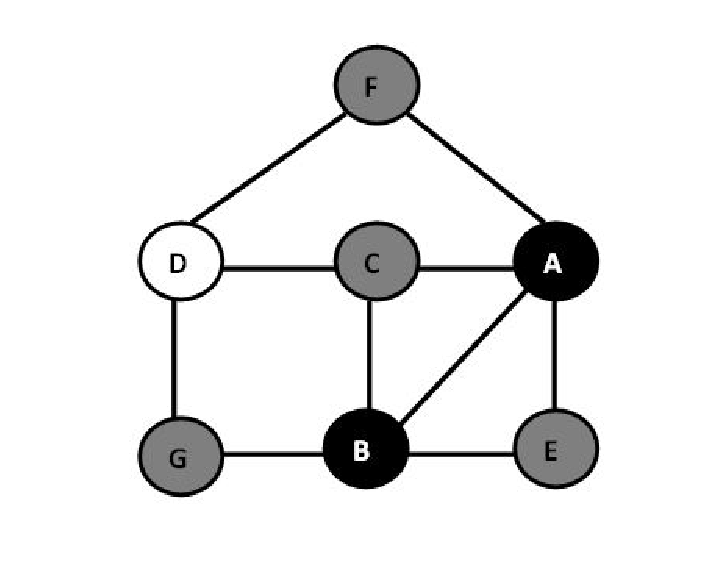
\includegraphics[width=0.9\linewidth,height=.8\linewidth]{Figures/cacds3.eps}
\\(c): Node B is selected and the process continues
\end{minipage}%
\begin{minipage}{.25\textwidth}
\centering
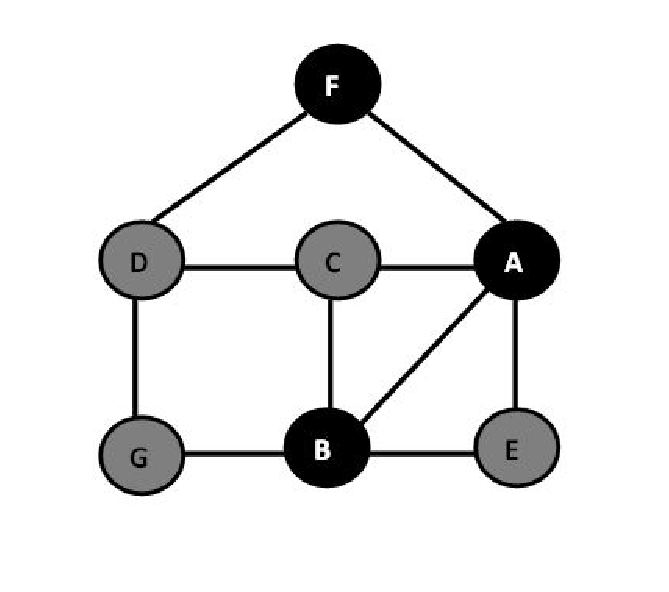
\includegraphics[width=0.9\linewidth,height=.8\linewidth]{Figures/cacds4.eps}
\\(d): Finally node A,B,F constructs the CACDS
\end{minipage}
\caption{ Step by step construction of Centralized Contention aware Connected Dominating Set (Centralized CACDS).}
\label{cds}
\end{figure*}

\subsection{Centralized Contention Aware Connected Dominating Set}
The centralized algorithm is presented in Algorithm \ref{Algorithm1}.
At the start of the algorithm, all the nodes are colored white and placed in $ColorW$ set. That means, $ColorW$ set consists of all nodes $v \in V$. 
%Whenever a node is selected as a forwarding node, the node and all its 1-hop neighbors are discarded from $ColorW$ set. 
The node with the maximum cardinality is then selected from $ColorW$ set and colored as black and placed in a different $ColorB$ set (shown in line 5-6 of Algorithm \ref{Algorithm1}). In case of tie, a node is selected randomly among the ones with maximal cardinality. All the neighbors of that black node are colored as gray and put the in $ColorG$ set. 
%The nodes in $ColorB$ set are the forwarding nodes of the network. When a node $ u \in ColorB$ forwards any message, all of its 1-hop neighbors receive the message and become member of $ColorG$ set. 
Among the gray nodes of $ColorG$ set, the nodes that have minimum number of black neighbors are selected and placed in a set called \textit{$Candidate\_Set$} (shown in line 17-22 of Algorithm \ref{Algorithm1}). The black nodes are already in CDS. Therefore, by selecting a gray node with minimum black neighbors reduces the chance of contention. 
In case of tie,
%Among the nodes in \textit{$Candidate\_Set$} 
the gray node which has maximum number of white neighbors is  selected and colored as black and all its white neighbors are colored as gray (shown in line 23-29 of Algorithm \ref{Algorithm1}) . A recursive selection process runs till there is no white node left in the network. 

The entire selection process is shown using the following example. Consider Figure \ref{cds}, among all the nodes node A has the maximum cardinality (which is 4 here), so, according to the algorithm, node A is colored black and all its neighbors (node B,C,E and F) are colored gray (illustrated in Figure \ref{cds}(b)). In the next step, all the gray nodes have only 1 black neighbor that is node A and each of the gray nodes B, C and F has 1 white neighbor and node E has none. So we can select either of Node B, C , F. Suppose, node B is selected to cover node G and it is colored as black and node G is colored as gray (illustrated in Figure \ref{cds}(c)). The only white node remaining in the network at this stage is node D. The gray node C has now two black neighbors (node A and node B), gray node G and node F each has one black neighbor, so either of node G and node F can be selected. Suppose node F is selected to cover node D ( In Figure \ref{cds}(d)). So, the final Contention aware Connected Dominating Set consists of node A,B and F. So, $$CACDS = \{A,B,F\}$$.
\begin{algorithm}

\caption{Centralized CACDS}
\label{Algorithm1}

\begin{algorithmic}[1]
 \STATE INPUT: G(V,E)
 \STATE RESULT \{CACDS\}
\STATE $ColorB=\emptyset$, $ColorG=\emptyset$, $CACDS=\emptyset$,
\STATE $ColorW$ = all nodes $v\in V$;
\STATE Select a node v $\in$ V with max(degree(v));
\STATE $ ColorB = \{v\} $;
\STATE $ ColorG= N(v)-\{v\}$;
\STATE $ ColorW=ColorW-N(v)$;


\WHILE{$ ColorW \neq \emptyset $}
 
   \STATE $MaxWhite=0$, $MinBlack=\|V\|$, $Candidate\_Set=\emptyset$;
 
        \FORALL{node $u \in ColorG$}
        
            \STATE $BlackCount = \|N(u) \cap ColorB\|$;
            \IF{$ BlackCount < MinBlack $}
                \STATE $MinBlack= BlackCount$;
            \ENDIF
        \ENDFOR
        \FORALL{ node $u \in ColorG$}
        
            \STATE $ BlackCount = \|N(u) \cap ColorB\|$;
            \IF{$BlackCount==MinBlack$}
           \STATE $ Candidate\_Set = Candidate\_Set \cup \{u\} $;
            \ENDIF
        \ENDFOR
            \FORALL{ node $w \in$ $Candidate\_Set$}
                \STATE $ WhiteCount = \|N(w) \cap ColorW\|$;
                \IF{$WhiteCount > MaxWhite$}
                 \STATE  $MaxWhite= WhiteCount$ ;
                 \STATE $selectedNode=w$;
                \ENDIF
            \ENDFOR
            
               
            \IF{$MaxWhite > 0$} 
                \STATE $ ColorB = ColorB \cup \{selectedNode\}; $ 
                \STATE $ColorW = ColorW-N(selectedNode)$; \\
                \STATE $ ColorG = ColorG \cup (N(selectedNode)-ColorB); $
            \ELSE
                \STATE $ColorG = ColorG - Candidate\_Set$;
            \ENDIF
            
\ENDWHILE
\STATE $ CACDS= ColorB$;

\end{algorithmic}
\end{algorithm}


\noindent{\bf Complexity Analysis of Centralized CACDS:}
In the algorithm \ref{Algorithm1}, the iteration of the $While Loop$ (line 9-37 of Algorithm \ref{Algorithm1}) continues until $ColorW$ set does not become empty. At first set $ColorW$ consists of all nodes in the network. So, the loop body will run in $O(V)$ times where $V$ is the total number of nodes in the network. Inside the $While Loop$, there are loops that are used to find the nodes which have minimum number of black neighbors and maximum number of white neighbors each of which individually runs in $O(V)$ times in the worst case scenario. So, the run time complexity of the Centralized CACDS is $O({V}^2)$.

\noindent{\bf Theoretical Correctness of CACDS:}
Next, we show the theoretical correctness of CACDS in the following two lemmas.

\textit{Lemma 1:} $CACDS$ is a connected dominating set.\\
\textit{Proof:} 
%Let us use contradiction to prove that $CACDS$ is a connected dominating set.
The proof is by contradiction.
Suppose the vertex set of CACDS is, $$V_{CACDS} = \{v_1,v_2,v_3...v_m\}$$
Assume node $v\textsubscript{i} \in V_{CACDS}$ cannot communicate with other nodes in $CACDS$. %and $cacds$ is the number of nodes in the $CACDS$.  
According to the algorithm, the black nodes are selected among the gray nodes. When a node becomes gray, that means it has at least one black neighbor in the network. As $v_i$ is a member of $CACDS$, the node must be black. When $v_i$ was selected, it was among one of the gray nodes and each gray node is connected to one of the black nodes. Therefore, each black node has at least one path to communicate with other nodes in $CACDS$. The result contradicts with the hypothetic premises. So, $v_i$ must have a path to connect other nodes in the $CACDS$. Hence each node in $CACDS$ must be connected. 

\textit{Lemma 2:} The connected dominating set constructed by $CACDS$ covers all the nodes in the network.\\
\textit{Proof:} Assume that, $U$ is the set consisting of all the nodes in the network, $U = \{x\textsubscript{1},x\textsubscript{2},...x\textsubscript{n}\}$, $n$ is the number of nodes in the network, and vertex set of CACDS is $V_{CACDS} = \{v_1,v_2,v_3...v_m\}$,
%$CACDS = \{v\textsubscript{1},v\textsubscript{2},v\textsubscript{3}...v\textsubscript{cacds}\}$
where $m$ is the total number of nodes in the $CACDS$. $N(v\textsubscript{i})$ is the set of nodes which become gray after selecting $v\textsubscript{i}$ as a member of $CACDS$ i.e., $N(v\textsubscript{i})$ represents the set consisting of all adjacent nodes of $v\textsubscript{i}$.\\
\begin{equation}
N = N(v\textsubscript{1}) \cup N(v\textsubscript{2}) \cup N(v\textsubscript{3}) \cup ... N(v\textsubscript{m})
\end{equation}
In order to prove, $CACDS$ covers all the nodes in the network, we have to prove that $U = N$.
As $CACDS$ is a connected dominating set, so every node $x\textsubscript{i} \in U$  either same as $v\textsubscript{j}$ or is adjacent to $v\textsubscript{j}$ for some $j$. In other words the following proposition must hold, 
$$ \forall i \Big[\exists j \big[x_i \in N(v_j) \big] \Big]$$
%Let $x\textsubscript{1} \in N(v\textsubscript{1})$;  $x\textsubscript{2} \in N(v\textsubscript{2})$; $x\textsubscript{n} \in N(v\textsubscript{m})$  
Thus,

\begin{equation}
    \{x\textsubscript{1},x\textsubscript{2},...x\textsubscript{n}\} \subseteq N(v\textsubscript{1}) \cup N(v\textsubscript{2}) \cup N(v\textsubscript{3}) \cup ... N(v\textsubscript{m}) 
    \label{eqn1}
\end{equation} 
From Equation \ref{eqn1},
\begin{equation}
   \{x\textsubscript{1},x\textsubscript{2},...x\textsubscript{n}\} \subseteq N
   \label{eqn2}
\end{equation}
By definition,
\begin{equation}
    \{x\textsubscript{1},x\textsubscript{2},...x\textsubscript{n}\} \subseteq U
    \label{eqn3}
    \end{equation}
 From Equation \ref{eqn2} and \ref{eqn3}, by the axiom of extensionality, we can say that, \\  
    \begin{equation}
\forall x_i (x_i \in U \Longleftrightarrow x_i \in N) \implies U = N
 \end{equation}

\subsection {Distributed Contention aware Connected Dominating Set (Distributed CACDS)}

For distributed CACDS, it is assumed that, each node knows its 2-hop neighborhood information. After receiving a packet from node $u$, if node $v$ finds itself in node $u$'s \textit{forward list}, it starts to make its own \textit{forward list} ($F\textsubscript{v}$) from a subset of its one-hop neighbors ($B\textsubscript{v}$) to cover all of its uncovered two-hop neighbors ($U\textsubscript{v}$). The sets $U_v$ and $B_v$ is calculated using the following equations:
% \begin{equation}
$$U\textsubscript{v} = N(N(v)) - N(v) - N(u)$$
%\end{equation}
%\begin{equation}
$$B\textsubscript{v} = N (v)- N (u) $$
%\end{equation}

 \begin{figure*}[h]
\begin{minipage}{.33\textwidth}
\centering
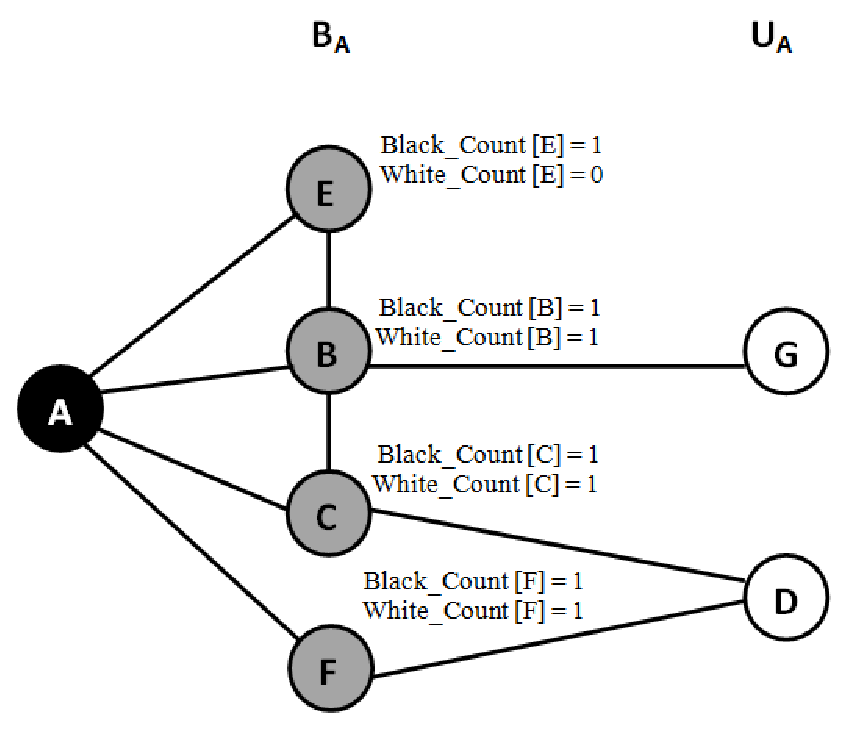
\includegraphics[width=0.8\linewidth,height=.7\linewidth]{Figures/dis1.eps}%
\\(a): Connection of node A with B\textsubscript{A} and U\textsubscript{A}
\end{minipage}%
\begin{minipage}{.33\textwidth}
\centering
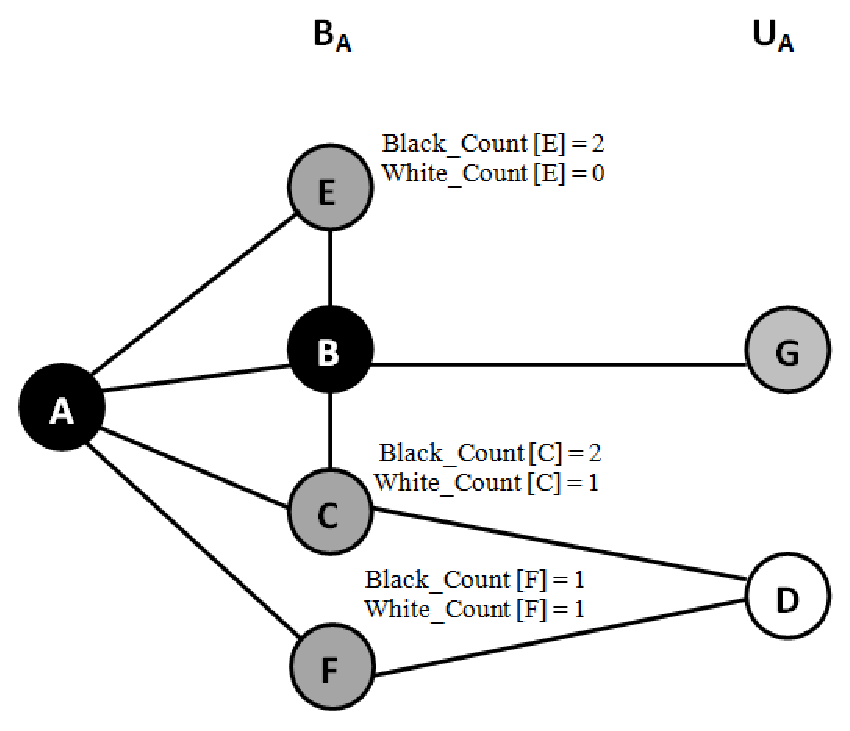
\includegraphics[width=0.8\linewidth,height=.7\linewidth]{Figures/dis2.eps}
\\(b): Node B is selected for F\textsubscript{A}
\end{minipage}
\begin{minipage}{.33\textwidth}
\centering
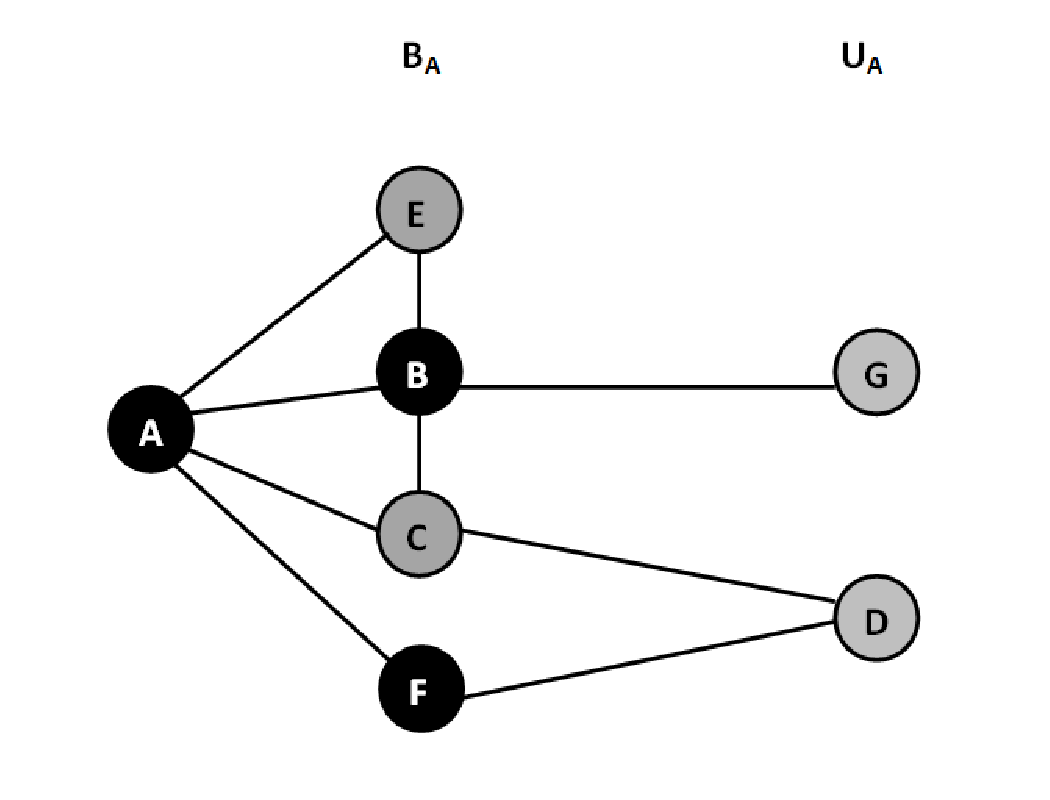
\includegraphics[width=0.8\linewidth,height=.7\linewidth]{Figures/dis3.eps}
\\(c): Node F finally selected for F\textsubscript{A}
\end{minipage}
\caption{ Step by step construction of Forward\_list of node A }
\label{dis}
\end{figure*}

 The new approach is stated in Algorithm 2. In the algorithm, an array named $Black\_Count$ is used so that each node  $p \in B\textsubscript{v}$ can keep track of its adjacent nodes in $B\textsubscript{v}$  that are already selected in the \textit{forwarding list}. At the start of constructing $F\textsubscript{v}$,  the corresponding value in the $Black\_Count$ array of all the nodes $p \in B\textsubscript{v}$ is set to one. The nodes whose corresponding value of the $Black\_Count$ is minimum among all the nodes in $B\textsubscript{v}$ are placed into a $Candidate\_Set$ (shown in line 13-17 of Algorithm \ref{Algorithm2}). Then in each iteration, a node $x \in Candidate\_Set$ is selected which covers maximum number of nodes in $U\textsubscript{v}$, i.e., $\|N(x) \cap U\textsubscript{v}\|$ is maximized (shown in line 18-30 of Algorithm \ref{Algorithm2}). Next, node $v$ includes node $x$ in its forwarding list $F\textsubscript{v}$ and the corresponding values of the $Black\_Count$ of the nodes in $B\textsubscript{v}$ adjacent to $x$ are all increased by one (shown in line 32-36 of Algorithm \ref{Algorithm2}). Node $v$ then updates $U\textsubscript{v} = U\textsubscript{v} - N(x)$  and $B\textsubscript{v} = B\textsubscript{v} - x$. This process is iterated until all nodes in $U_v$ is covered or no change in $B_v$ set is possible.

Let us explain the process using an example scenario. Consider Figure \ref{cds}. Suppose node A is the broadcast initiator. Figure \ref{dis} is the redrawing of Figure \ref{cds} for better visualization in order to determine the \textit{forward\_list} of node A. $B\textsubscript{A}$ consists of node B, C, E and F and $U\textsubscript{A}$ consists of node D and G. In DP, node A selects node B and C for forwarding the message to cover node G and D. This selection arises contention between node B and node C when they start to rebroadcast.

The proposed algorithm aims at minimizing this type of contention. The algorithm does not select node C to cover node D if node A decides to choose node B to cover node G. It selects node F instead to cover node D to avoid contention. So, node B and F will be in the forward list of node A. Hence, $F\textsubscript{A}=\{B,F\}$. The whole process is shown in Table \ref{table:5}.
\begin{algorithm}
\caption{Creation of forward\_list of a node $v$}

\label{Algorithm2}
\begin{algorithmic}[1]
\STATE $Forwarding\_node \leftarrow v$
\STATE $F\textsubscript{v} = \emptyset$, $size\_of\_forward\_list=0$,

 \FORALL{node $p \in B\textsubscript{v}$}
    \STATE $Black\_Count[p] = 1$;
 \ENDFOR
\WHILE{$ U\textsubscript{v} \neq \emptyset $ or $B_v$ remains unchanged}
    \STATE $maximum = 0$, $minimum=\|V\|$, $Candidate\_Set=\emptyset$;
    
    \FORALL{node $q \in B\textsubscript{v}$}
        \IF{$Black\_Count[q] < minimum$}
            \STATE $minimum = Black\_Count[q] $;
        \ENDIF
    \ENDFOR
     \FORALL{node $r \in B\textsubscript{v}$}
        \IF{$ Black\_Count[r] == minimum $}
            \STATE $Candidate\_Set = Candidate\_Set \cup \{r\}$;
        \ENDIF
     \ENDFOR
     
     \FORALL{node $s \in Candidate\_Set$}
        \FORALL{node $t \in U\textsubscript{v}$}
            \IF{node $t \in N(s)$}
                \STATE $ White\_Count[s] = White\_Count[s]+1 $;
            \ENDIF
        \ENDFOR
    \ENDFOR
    
     \FORALL{node $i \in Candidate\_Set$}
        \IF{$White\_Count[i] > maximum$}
            \STATE $maximum = White\_Count[i]$;
            \STATE $x = i$;
        \ENDIF
    \ENDFOR
     \IF{$maximum > 0$}   
     \STATE $F\textsubscript{v}[size\_of\_forward\_ list] = \{x\}$;
     \STATE $size\_of\_forward\_ list = size\_of\_forward\_ list + 1$;
     \FORALL{node $y \in (B\textsubscript{v} \cap N(x))$}
        \STATE $ Black\_Count[y]= Black\_Count[y]+1$;
    \ENDFOR
     \STATE $ U\textsubscript{v} = U\textsubscript{v} - N(x)$;
      \STATE $B\textsubscript{v} = B\textsubscript{v}-\{x\}$;
     \ENDIF
\ENDWHILE
\end{algorithmic}
\end{algorithm}
\begin{table}[h]

  \begin{center}
    \caption{Forwarding lists creation process in Distributed CACDS algorithm for the scenario of Figure \ref{cds}(a) (node A is the source of broadcast)}.
     \medskip
    \label{table:5}
    \renewcommand{\arraystretch}{1}
       \begin{tabular} {|>{\centering\arraybackslash}p{1cm}|>{\centering\arraybackslash}p{1cm} |>{\centering\arraybackslash}p{1.5cm} | >{\centering\arraybackslash}p{2cm}|>{\centering\arraybackslash}p{1cm}|}
      \hline
      \bf{Previous node ($u$)} & \bf{Current node ($v$)} & \bf{$U\textsubscript{v}$} & \bf{$B\textsubscript{v}$} & \bf{$F\textsubscript{v}$} \\
      \hline
      $\emptyset$ & A &\{B,C,E,F\} &\{G,D\} &\{B,F\} \\
      \hline
      A  & B  & \{G\}& \{D\} & \{G\}  \\
      \hline
      A  & F  & \{D\} & \{G\} & \{D\}  \\
      \hline
      B  & G & \{D\} & \{F\} & \{D\} \\
      \hline
      F  & D &\{C,G\}& \{B\} & \{C\}    \\
      \hline
      D  & C & \{A,B\} & \{E\}& \{A\}   \\
      \hline
    
    \end{tabular}

  \end{center}
\end{table}

\noindent{\bf Complexity Analysis of Distributed CACDS:}
Constructing the $forwarding\_list$ of a node $v$ is very much similar to set cover problem.  Suppose, the maximum degree of a node is $\Delta$. In the worst case scenario the size of $B\textsubscript{v}$ set of a node v can be equal to $\Delta$, i.e. $|B\textsubscript{v}| = \Delta$. Forwarding nodes should be chosen from the set $B\textsubscript{v}$ to cover the nodes that belong to set $U\textsubscript{v}$. The maximum number of nodes in $U\textsubscript{v}$ set that can be covered by $B\textsubscript{v}$ is $\Delta^2$. So, final run time of constructing the $forwarding\_list$ of node $v$ is $O(\Delta^3)$.

